\chapter{Knowledge}
\label{cha:knowledgei}

\section{Prerequisites}

This section will introduce some important knowledges, including sigmoid function, Bayes Formula and Huffman code etc.

\subsection{Sigmoid Function}

Sigmoid Function is a common kind of active function, the definition is

$$ \sigma(x) = \frac{1}{1+e^{-x}} $$,

The domain is $(-\infty, \infty)$, the range is $(0,1)$.

\begin{figure}[H]
\centering
\begin{minipage}{.4\textwidth}
  \centering
	\fbox{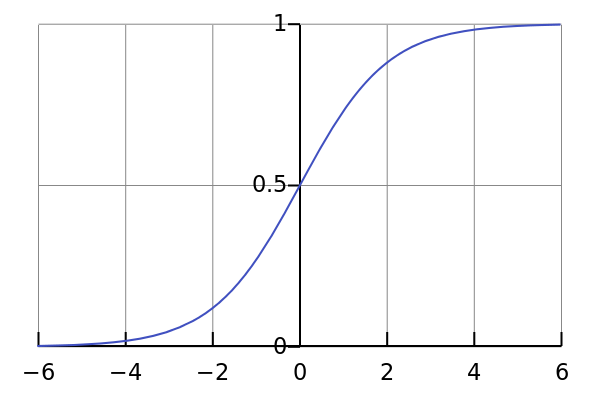
\includegraphics[width=0.95\textwidth]{sigmoid} }
	\caption{Sigmoid Function}
	\label{fig:sigmoid}
\end{minipage}
\end{figure}

sigmoid function has the \textbf{}

\subsection{And some controversy}



%--------------------------------------------------------------------------------------------------------------------------------%

\section{Skip-gram model}


\subsection{Softmax function}


\subsection{Hierarchical Softmax}


\subsection{Negative Sampling}

